\section{问题二的分析与求解}

\instruction{本节占位。问题二：恒温干燥阶段（附录 3 变物性：$\rho$、\cp、\kcond、\Ddiff 均为 \C、\T 的函数）。由 @model 提供公式、@impl 求解、@paper 排版。}

\subsection{模型的建立}
\instruction{变物性控制方程、表面对流换热 + 蒸发潜热耦合边界条件占位。}

\subsection{模型的求解}
\instruction{非线性/变物性的离散与迭代策略占位。}

\subsection{结果与分析}
\instruction{结果表/图由 scripts 生成。表编号以 scripts/make\_tables.py 输出为准，此处仅占位。}

% 表格片段本身已是完整的 table 环境（含 \caption 与 \label），
% 故此处**不再套一层 table**，否则会嵌套浮动体并与生成片段撞 label。
\IfFileExists{tab/q2_temp.tex}{%
  % 本文件由 scripts/make_tables.py 自动生成，请勿手工编辑
\begin{table}[htbp]
  \centering
  \caption{3 小时内药材的温度（°C；距离单位：cm）}
  \label{tab:q2-temperature}
  \begin{tabular}{cccccc}
    \toprule
    时间/h & 0 & 0.5 & 1 & 1.5 & 2 \\
    \midrule
    0.5000 & 30.9783 & 31.1516 & 31.6717 & 32.5411 & 33.7666 \\
    1.0000 & 37.1509 & 37.2577 & 37.5696 & 38.0616 & 38.6817 \\
    1.5000 & 40.0220 & 40.0621 & 40.1787 & 40.3628 & 40.5741 \\
    2.0000 & 41.0667 & 41.0816 & 41.1257 & 41.1953 & 41.2476 \\
    2.5000 & 41.4202 & 41.4249 & 41.4382 & 41.4593 & 41.5048 \\
    3.0000 & 41.5644 & 41.5658 & 41.5724 & 41.5833 & 41.5617 \\
    \bottomrule
  \end{tabular}
\end{table}
%
}{%
  \instruction{表占位：tab/q2\_temp（scripts/make\_tables.py 生成）尚未生成。}
}

\IfFileExists{tab/q2_moist.tex}{%
  % 本文件由 scripts/make_tables.py 自动生成，请勿手工编辑
\begin{table}[htbp]
  \centering
  \caption{3 小时内药材的水分浓度（kg/kg；距离单位：cm）}
  \label{tab:q2-moisture}
  \begin{tabular}{cccccc}
    \toprule
    时间/h & 0 & 0.5 & 1 & 1.5 & 2 \\
    \midrule
    0.5000 & 2.5500 & 2.5499 & 2.5483 & 2.5371 & 2.5011 \\
    1.0000 & 2.5488 & 2.5471 & 2.5386 & 2.5093 & 2.4243 \\
    1.5000 & 2.5411 & 2.5355 & 2.5131 & 2.4561 & 2.3385 \\
    2.0000 & 2.5202 & 2.5095 & 2.4723 & 2.3952 & 2.2621 \\
    2.5000 & 2.4855 & 2.4707 & 2.4231 & 2.3343 & 2.1956 \\
    3.0000 & 2.4411 & 2.4238 & 2.3701 & 2.2749 & 2.1310 \\
    \bottomrule
  \end{tabular}
\end{table}
%
}{%
  \instruction{表占位：tab/q2\_moist（scripts/make\_tables.py 生成）尚未生成。}
}

\begin{figure}[htbp]
  \centering
  \IfFileExists{figs/fig2-C-profiles.pdf}{%
    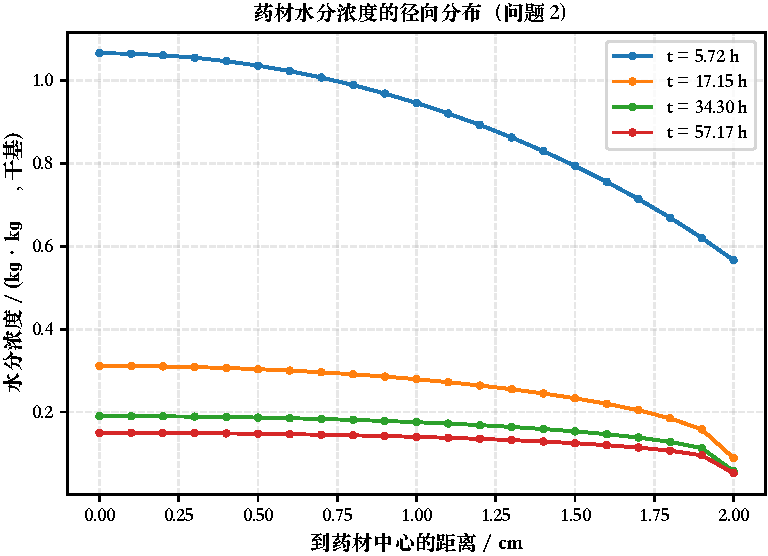
\includegraphics[width=0.75\linewidth]{figs/fig2-C-profiles.pdf}%
  }{%
    \instruction{图占位：figs/fig2-C-profiles.pdf 尚未生成（scripts/make\_figs.py）。}
  }
  \caption{恒温干燥阶段药材内部水分浓度分布}
  \label{fig:q2-concentration}
\end{figure}
